\section{Projektergebnisse}
In diesem Kapitel wird die prototypische Implementierung der Schnittstelle für die Anbindung von austauschbaren Datenquellen an KI-Algorithmen beschrieben.

\subsection{Softwarearchitektur}
Ein grundlegender Dienst, der Daten mit einer KI verbindet, kann mithilfe eines einzigen Python-Scripts erstellt werden. Die Herausforderung an einer praxistauglichen Anwendung, die gleichzeitig von mehreren Usern genutzt werden kann, liegt im  Architekturdesign der Software. Eine praxistaugliche Anwendung muss neben den funktionalen Anforderungen auch noch weitere nicht funktionale Anforderungen erfüllen. Die drei wichtigsten nicht funktionalen Anforderungen sind Performance, Skalierbarkeit und Verfügbarkeit. Alle drei Anforderungen können mit einem lokal ausgeführten Skript nicht erfüllt werden. 

Damit Nutzer mit der Software interagieren können, wird ein Frontend benötigt. Ein zentral gehostetes, webbasiertes Frontend kann von einem Nutzer über eine einfache \ac{url} im Webbrowser aufgerufen werden. Für die anzuzeigenden Daten im Frontend wird eine Verbindung zum Backend benötigt. Diese wird über eine HTTP Verbindung zur mit Flask gehosteten \ac{rest} API bereitgestellt.

Um die Anforderung der Skalierbarkeit erfüllen zu können, ist die REST-API komplett zustandslos implementiert worden. Eine API ohne Zustände speichert keine Zwischenstände zu den Anfragen einzelner Nutzer. Bei jeder Anfrage an die API müssen alle Informationen im Request bereitgestellt werden, die die API zum bearbeiten der Anfrage benötigt. Dies bietet die Möglichkeit bei steigender Nutzerzahl mehrere parallel betriebene Instanzen der API hochzufahren. Dadurch ist eine horizontale Skalierung gewährleistet. Horizontal skalierbare Instanzen innerhalb der Software Architektur sind in Abbildung 1 mit zwei hintereinander gestapelten Rechtecken visualisiert.

Da die Kommunikation zwischen dem Frontend, der API und den KI-Services asynchron läuft, muss das Flask Backend trotz seiner Zustandslosigkeit Transformationsanleitungen und Ergebnisse der KI-Services zwischenspeichern, bis sie im Frontend benötigt werden. Um die Performanceanforderungen erfüllen zu können, können nicht alle Zwischenstände in einer MySQL Datenbank gespeichert werden. Die Lese- und Schreibgeschwindigkeit kann bei steigender Nutzerzahl problematisch werden. Um dem Entgegenzuwirken wird ein Redis Key-Value Store als Cache betrieben. Die zwischengespeicherten Daten werden nach dem ersten Aufruf wieder gelöscht, weswegen eine persistente Speicherung nicht notwendig ist. In-Memory Datenbanken speichern und führen ihre Queries direkt im RAM aus, wodurch Anfragen im Vergleich zu einer MySQL Datenbank deutlich schneller ausgeführt werden.

Im Flask Backend werden alle Routen und die meisten Funktionen abgekapselt in einem Funktion Wrapper ausgeführt. Dieser fungiert als eine Art Sandbox, in der auftretende Fehler nicht zum Programmabsturz führen, sondern behandelt und geloggt werden können. Alle Logs werden persistent in einer MySQL Datenbank gespeichert. Mit dem Dienst Grafana können diese Logs angezeigt werden.

Die Laufzeit von KI-Services kann sehr stark vom verwendeten KI-Modell, der zu durchsuchenden Datenmenge, wie auch der vom Nutzer gesendeten Eingabe abhängen. Bei einer synchronen Kommunikation zwischen dem Flask Backend und dem Service können sehr lange Wartezeiten entstehen. Wenn der KI-Service ebenfalls eine REST-Schnittstelle implementieren würde, könnten es bei einem HTTP Request zum Timeout der Anfrage führen. Aufgrund der schwanken Laufzeit muss eine asynchrone Kommunikationsstruktur, wie RabbitMQ mit dem AMQP implementiert werden.

Die einzelnen Services können mit einem Eintrag in der MySQL Datenbank registriert werden. Für die Registrierung muss lediglich der Name und der im Frontend anzuzeigende Name des Services hinterlegt werden. Die Registrierung eines Dienstes kann durch den Aufruf einer Route in der API durchgeführt werden. 

Der im Prototypen implementierte KI-Service nutzt das BERT Modell von Google zum konvertieren der Nutzereingaben in semantische Vektoren. Es wird ebenfalls eine Elasticsearch Datenbank betrieben, in der alle zu Durchsuchenden Einträge gespeichert sind. Im Gegensatz zu einer MySQL Datenbank, kann in einer Elasticsearch Datenbank zu jedem Eintrag ein semantischer Vektor gespeichert werden. Der KI-Service kann mithilfe der Kosinusähnlichkeitssuche den semantischen Vektor der Eingabe mit den Vektoren der Datenbank vergleichen und so die semantisch ähnlichstes Texte herausfiltern. Die gefunden Einträge werden über RabbitMQ im Anschluss wieder an das Flask Backend geschickt, damit sie dort vom Frontend ausgelesen werden können.

\begin{figure}[H]
  \centering
    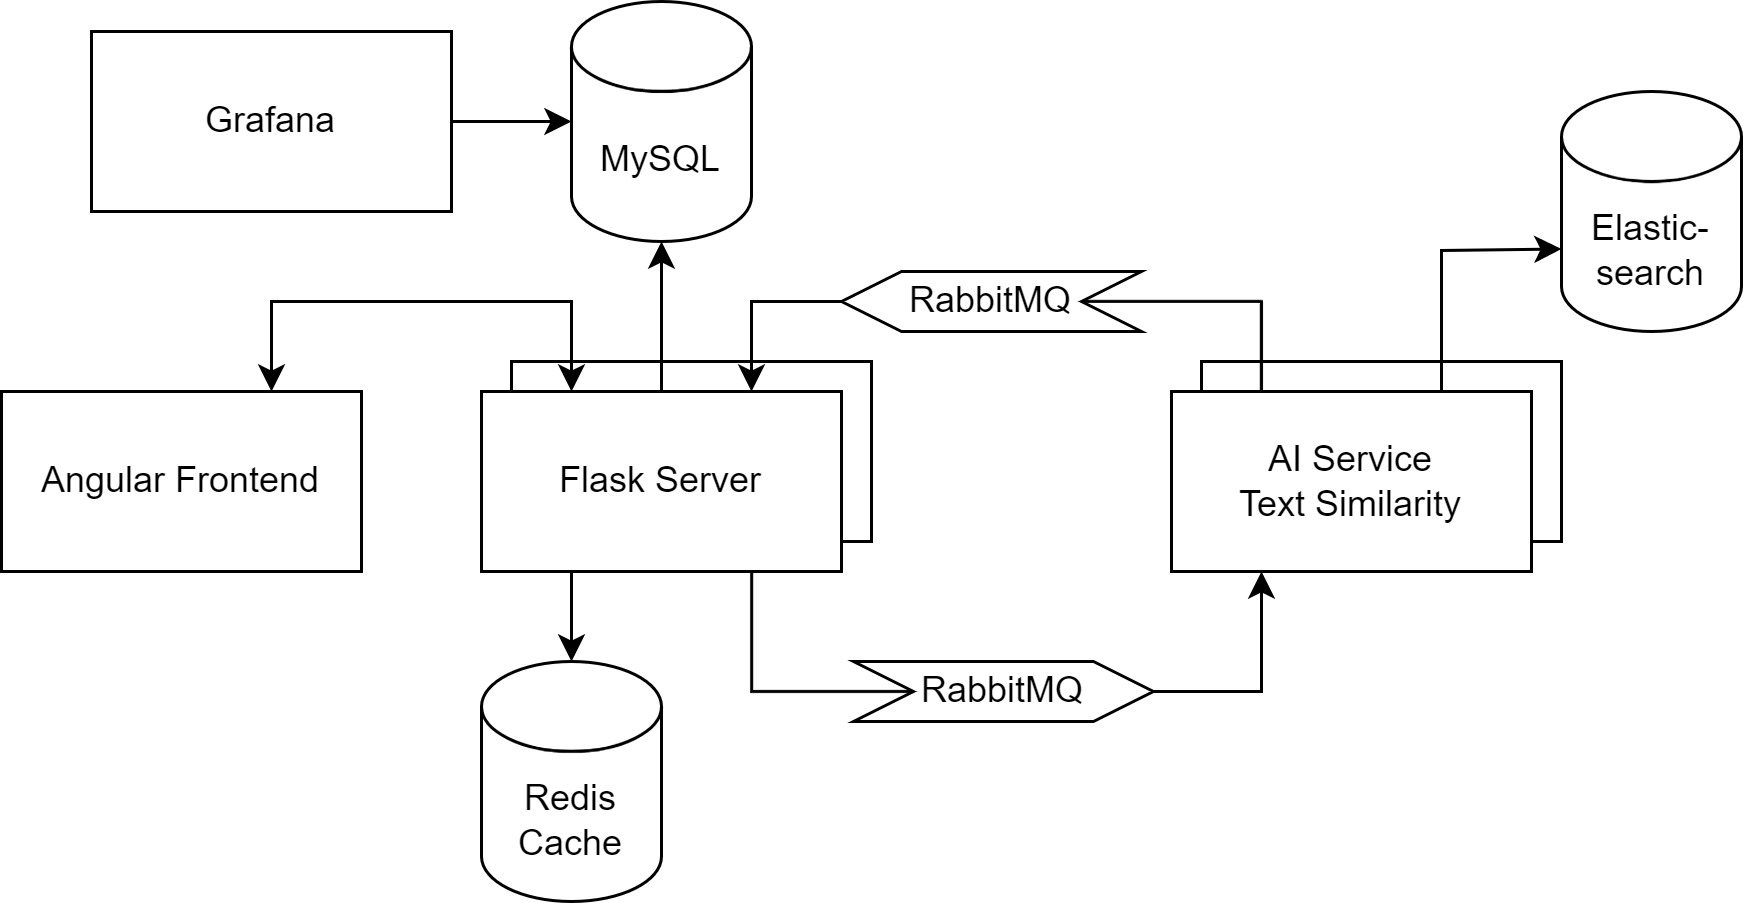
\includegraphics[width = 15cm]{bilder/Architektur}
    \caption{Softwarearchitekturdiagramm}
\end{figure}

\subsection{REST-API mit Flask}
Eine API stellt einen Satz an Daten und Funktionen bereit, um den Austausch von Daten zwischen verschiedenen Programmen zu ermöglichen. REST ist ein Regelsatz, in dem die Form, Funktionalität und der Aufbau einer API beschrieben wird.\footcite{masse2011rest}
In einer REST-API werden mehrere Routen definiert. Die Funktion der Route sollte sich nach Möglichkeit implizit durch den Aufbau der URL und den Request Typ ableiten lassen. Die im Prototypen verwendeten Request Typen sind \texttt{GET}, \texttt{POST}, und \texttt{DELETE}. Im HTTP werden noch weitere Typen unterstützt, die in dieser Arbeit jedoch keine Verwendung finden. \texttt{GET} Requests haben keine Auswirkungen auf den Zustand oder die Daten auf dem Server. Es werden nur die aktuellen angeforderten Daten in der Reponse zurückgegeben. \texttt{POST} Requests können in ihrem Body Daten beinhalten, die auf die Bearbeitung des Requests Einfluss nehmen. Die Daten werden im Prototypen in Form von JSON Dokumenten an die API übergeben.

\subsubsection{Aufbau und Implementierung der REST-API}
Python bietet mit dem Package Flask die Möglichkeit einen simplen und gut skalierbaren Webserver aufzusetzen. Für das Starten einer Flask Instanz muss das Package Flask in die Python Umgebung importiert werden. Anschließend kann ein Flask-Objekt erzeugt und die Flask Instanz mit den gewünschten Parametern gestartet werden.

\begin{lstlisting}[language=Python]
from flask import Flask
app = Flask(__name__)
app.run(host="0.0.0.0", port=80, use_reloader=False)
\end{lstlisting}

Damit die API auch automatisiert aus einem Docker Container heraus gestartet werden kann, muss die Ausführung des Flask Services in die Main Methode von Python ausgelagert werden. Flask blockiert den Thread auf dem es ausgeführt wird, was eine asynchrone Kommunikation über RabbitMQ nicht möglich macht. Der Receiver benötigt seinen eigenen Thread, weswegen eine Multithreading-Architektur implementiert werden muss. Zu diesem Zweck wird das threading Package genutzt. Über den Parameter \texttt{daemon} kann bei der Erzeugung eines Threads festgelegt werden, dass der Thread im Hintergrund läuft und den Hauptthread nicht blockiert.

\begin{lstlisting}[language=Python]
def start_server():
    app.run(host="0.0.0.0", port=80, use_reloader=False)

if __name__ == '__main__':
    thread_server = threading.Thread(target=start_server, daemon=True).start()
\end{lstlisting}

Eine in der API adressierbare Route kann in Flask über Function-Annotations definiert werden. Die von Flask implementierten Anntotations haben die Form \texttt{instanz.route('path', methods=["METHOD"])}. Der Name der Instanz wird am Anfang des Projekts als \texttt{app} definiert. Der \texttt{path} beschreibt die Route, die vom Frontend aufgerufen werden muss, damit die nachfolgende Funktion ausgeführt wird. Im Array \texttt{methods} besteht die Möglichkeit, ein oder mehrere Request Typen zu definieren, die die Funktion akzeptieren soll.

Eine beispielhafte Nutzung der Annotations, um eine Route in der API zu definieren, ist nachfolgend aufgeführt. 

\begin{lstlisting}[language=Python]
@app.route('/', methods=["GET"])
def index():
    [..]
    return r.respond({"token": token}, cookie=f"Authorization={token}")
\end{lstlisting}

Der Inhalt der Methode und deren genaue Funktionsweise wird in den folgenden Kapiteln näher erläutert.

Die Funktion \texttt{respond} ist im Skript \texttt{api/response\_{}generator.py} definiert. Sie dient als Function Wrapper, der bei jeder ausgehenden Response die Response-Header, eventuelle Cookies und den Reponse Typen setzt. Der Output der Response wird mithilfe des \texttt{json} Packages in JSON Syntax konvertiert.

\begin{lstlisting}[language=Python]
import json
from flask import Response
def respond(r, status=200, json_dump=True, cookie=""):
    [...]
    return Response(json.dumps(r), status=status, mimetype='application/json', headers=headers)
\end{lstlisting}

In Tabelle 1 sind alle in der API verfügbaren Routen aufgelistet. Auf die genaue Funktionalität der einzelnen Funktionen wird in den folgenden Kapitel eingegangen.

\begin{table}[H]
\centering
\begin{tabular}{c|c|l}
\textbf{Route} & \textbf{Typ} & \textbf{Funktion}\\
\hline
\texttt{'/'} & \texttt{GET} & Erstellung eines JSON Web Tokens\\
\hline
\texttt{'/upload/file'}  & \texttt{POST} & Hochladen einer Textdatei für den Input der KI \\
\texttt{'/upload/text'}  & \texttt{POST} & Texteingabe für den Input des KI-Services \\    
\texttt{'/transform'}  & \texttt{POST} & Festlegen der Tranformationseigenschaften\\ 
\texttt{'/send'}  & \texttt{POST} & Transformieren und Senden des Inputs an einen KI-Service \\ 
\texttt{'/poll'}  & \texttt{GET} & Abfrage der vom KI-Service gelieferten Ergebnisse \\ 
\hline
\texttt{'/service'}  & \texttt{GET} & Auflistung aller Services \\
\texttt{'/service'}  & \texttt{POST} & Registrieren eines neuen Services \\ 
\texttt{'/service'}  & \texttt{DELETE} & Löschen eines Services \\       
\end{tabular}
\caption{Implementierte Routen der REST-API}
\end{table}

\subsubsection{Nutzeridentifizierung mit JWT}
Innerhalb des Backendes ist es notwendig, einzelne Nutzer voneinander zu unterscheiden. Für jeden Nutzer speichert das Backend den hochgeladenen Text, die Transformationsanleitung und die Antworten des angefragten KI-Services im Redis Cache. Um Nutzer voneinander unterscheiden zu können, gibt es zwei grundlegende Möglichkeiten. 
\begin{enumerate}
\item Identifizierung durch den Nutzer der Software. Beispielsweise mittels Registrierung durch E-Mail Adresse und Passwort.
\item Identifizierung durch das Backendend der Software. Generierung und Zuweisung einer zufälligen aber eindeutigen User-ID.
\end{enumerate}

Die Erhebung von personenbezogenen Daten setzt die Einhaltung der \ac{dsgvo} voraus. Dies bedeutet einen erheblichen Mehraufwand für eine Anwendung, die sonst keinen weiteren Nutzen aus den Daten zieht.

Das Backend nutzt einen \ac{uuid} der sich durch das Python Package \texttt{uuid} generieren lässt. Eine UUID ist eine 32 Zeichen lange Zahl im Hexadezimalformat. Die importierte Funktion \texttt{uuid4()} erzeugt eine zufällige, ohne von Parametern beeinflusste UUID. Der Nutzer muss diese UUID mitgeteilt bekommen und für alle seine Anfragen, aufgrund der zustandslosen Implementierung der API, im Authorization Header mitschicken. Damit die UUID nicht ausgelesen oder manipuliert werden kann, wird sie nicht als einfacher Text in der Response an den Nutzer geschickt, sondern vorher in ein JSON Token geschrieben und verschlüsselt.

Ein \ac{jwt} ist ein kompaktes, URL-sicheres Mittel zur Darstellung von Forderungen, die zwischen zwei Parteien übertragen werden sollen. Die Angaben in einem JWT werden als JSON-Objekt kodiert. Der Inhalt des JST kann digital signiert oder die Integrität mit einem \ac{mac} geschützt und/oder verschlüsselt werden.\footcite{jones2015json}

Im nachfolgenden Codeausschnitt ist die Generierung der UUID und die Verschlüsselung des JWT dargestellt.
\begin{lstlisting}[language=Python]
def uuid_gen():
    return uuid.uuid4()
    
def encode_token(param):
    return jwt.encode(param, JWT_PASSWORD, algorithm="HS256")

token = encode_token({'uid': str(uuid_gen())})
\end{lstlisting}

Für jede Route, ausgenommen die \texttt{/service} Routen zum Management der Services, wird der JWT für die Ausführung benötigt. Die Überprüfung und Entschlüsselung des Tokens ist für jede Route gleich, daher ist es sinnvoll diese Funktionalität zu zentralisieren. Damit wird die Fehleranfälligkeit reduziert und und die Wartbarkeit erhöht, sollte sich zum Beispiel der Algorithmus oder das Passwort für die Verschlüsselung ändern. Wie auch Flask Annotations zum definieren einer Route verwendet, ist es möglich eigene Annotations zu entwerfen. Für diese Funktion ist das Python Package \texttt{functools} mit der Funktion \texttt{wraps} zuständig. Wraps ermöglicht es, Funktionen ineinander zu verschachteln.

Im Prototypen wird die Funktion \texttt{token\_{}required(f)} definiert. Diese Funktion dient als eine Umgebung, in der eine weitere Funktion ausgeführt werden. Im Gegensatz zur normalen Ausführung einer Funktion, werden in der \texttt{token\_{}required(f)} Funktion vor der Ausführung der eigentlichen Funktion mehrere Rahmenbedingungen geprüft. Der vom Nutzer gesendete Token muss nach der erfolgreicher Entschlüsselung syntaktisch korrektes JSON enthalten. Sollte dies nicht der Fall sein, wird die die eigentliche Funktion, die zur API Route gehört, gar nicht erst ausgeführt. Der Nutzer bekommt direkt eine Respose mit dem HTTP Error-Code 401: Unauthorized gesendet. \footcite{fielding1999rfc2616}

Wenn die Entschlüsselung des Tokens erfolgreich war, wird die innere Funktion ausgeführt. Als Parameter der inneren Funktion wird die im JWT enthaltene UUID übergeben. Durch diesen Aufbau ist der Code für die Verifizierung des Tokens und die Logik der Funktion unter der angesprochenen Route vollständig getrennt.

\begin{lstlisting}[language=Python]
@routes.route('/upload/text', methods=['POST'])
@token_required
def upload_text(uid):
    [...]
\end{lstlisting}

\subsubsection{Caching mit Redis Datenbank}
Redis ist ein Key-Value Store der vollständig im RAM ausgeführt wird. Innerhalb von Redis sind mehrere Datenbanken definiert, die in ihrer Standartkonfiguration über einen Index $i$, mit $0\leq{}i<16$ aufgerufen werden. Im Backend werden die ersten drei Datenbanken verwendet.
\begin{enumerate}
 \item Datenbank 0: Cache der hochgeladenen Textdateien für den Input der KI
 \item Datenbank 1: Cache der Transformationsanleitung
 \item Datenbank 2: Cache der vom KI-Service produzierten Ergebnisse
\end{enumerate} 


\subsubsection{Management der Services}
text
\subsubsection{Automatisierte Transformation des Inputs}
text
\subsubsection{Fehlerbehandlung}
Während des Laufzeit des Programms kann es dazu kommen, dass im vom Nutzer produzierte Fehler auftreten. Der Nutzer kann im Bereich der Transformation syntaktisch nicht korrekte Texte eingeben, die Backend verarbeitet werden. Da Nutzereingaben ohne weitere Behandlung ebenfalls ein Sicherheitsrisiko für die Infrastruktur darstellen können, wird im Backend ein System implementiert, um die Verarbeitung der Eingaben in einer isolierten Umgebung ausführen zu können. Ähnlich wie bei der Verifizierung des JWT, ist das System zur Fehlerbehandlung auch mit Function Wrappern und Annotations umgesetzt. 

Im Backend wird ein Exception Handler definiert der eine Funktion mit zuvor übergebenen Parametern ausführt. Da eine fehlerhafte Ausführung auch dort zum Programmabsturz führen würde, wird die Funktion in einem try-except Block gekapselt. Alle innerhalb dieses Blocks auftretende Fehler werden abgefangen und in einem Exception Objekt gespeichert. Innerhalb des Exception Objekts ist die produzierte Fehlermeldung gespeichert. Über \texttt{str(e)} kann auf die Fehlermeldung zugegriffen werden. Innerhalb des Except Blocks wird die Fehlermeldung an den Logger weitergegeben, um diese in einer Datenbank persistent zu speichern. Nach erfolgreichem Log wird dem Frontend in einer HTTP Response der Statuscode 500 \glqq Internal Server Error\grqq{} zurückgegeben.\footcite{fielding1999rfc2616}

\begin{lstlisting}[language=Python]
[...]
 @wraps(f)
        def decorator(*args, **kwargs):
            try:
                return f(*args, **kwargs)
            except Exception as e:
                logger.log("error", f"[Server, {msg}]: {str(e)}", "none")
                return r.respond({"success": False, "error": str(e)}, status=500)
            [...]
\end{lstlisting}

Jede Funktion, die in innerhalb des Exception Handlers ausgeführt werden soll, wird mit der Annotation \texttt{@exception\_{}handler("...")} versehen. Innerhalb des Parameters, wird der Ort, an dem die Funktion ausgeführt wird, und damit der Fehler auftritt, als String übergeben. Diese Information wird genutzt, um innerhalb des Fehlerlogs den Ort des Fehlers aufzulisten.

\subsubsection{Event Logging}
Das Backend implementiert ein Event Logging System mit dem Zustände und Informationen des Systems in einer Datenbank gespeichert werden können. Mithilfe von Logs können Entwickler den Ablauf eines Programms besser nachvollziehen und auftretende Fehler schneller zu ihrer Quelle zurückverfolgen. Es ist ebenfalls möglich, Systeme aufzusetzen, die die auf Logs auslesen und beim Auftreten eines Errors die zuständigen Personen alarmieren. Eine Herausforderung bei einem Logging System ist es, dass das System dem Entwickler beim Loggen keinen erheblichen Mehraufwand produzieren soll. Im Backend wurde ein Logging System entwickelt, welches mit einer einzigen Funktion angesteuert werden kann. Die Log Funktions des Loggers wird in den verschiedenen Bereichen der Anwendung über \texttt{from logs.logger import log} importiert. Nach erfolgreichem Import, steht die \texttt{log} Funktion zur Verfügung. 

Für einen Log müssen drei Parameter übergeben werden, der Log Level, eine Message und die UUID. Die möglichen Ausdrücke für die Log Level sind in Tabelle 2 aufgeführt. Die unterstützten Log Level leiten sich aus der Funktionalität von Grafana ab, welche diese Logs mit einer zugeordneten Farbe visualisiert.

\begin{table}[H]
\centering
\begin{tabular}{c|c|c}
\textbf{Ausdruck} & \textbf{Log Level} & \textbf{Farbe}\\
\hline
emerg & critical & lila\\
fatal & critical & lila\\
alert & critical & lila\\
crit & critical & lila\\
critical & critical & lila\\
err & error & rot\\
eror & error & rot\\
error & error & rot\\
warn & warning & gelb\\
warning & warning & gelb\\
info & info & grün\\
information & info & grün\\
notice & info & grün\\
dbug & debug & blau\\
debug & debug & blau\\
trace & trace & hellblau\\
* & unknown & grau
\end{tabular}
\caption{Log Level des Event Logging Systems}
\end{table}

Innerhalb der Log Funktion wird eine Datenbank Query mit den drei Parametern und einem aktuellen Zeitstempel erstellt. Der Zeitstempel kann mithilfe des \texttt{datetime} Packages erstellt werden. Über \texttt{cursor.execute()} wird die erstellte Query in der MySQL Datenbank ausgeführt. Der Log wird als Eintrag in der Tabelle \texttt{logs} gespeichert. 

\begin{lstlisting}[language=Python]
def log(level, message, uid):
    [...]
    query = f"INSERT INTO logs (`level`, `message`, `timestamp`, `uid`) VALUES (%s, %s, %s, %s)"
    cursor.execute(query, (level, message, datetime.utcnow(), str(uid)))
    [...]
\end{lstlisting}

\subsection{Kommunikation zwischen Backend und Services mit RabbitMQ}
Für den Informationsaustausch zwischen dem Backend und den verschiedenen KI-Services ist eine asynchrone Kommunikation implementiert. Je nach Komplexität des Services, kann die Verarbeitung einer vom Nutzer gestellten Anfrage mehrere Sekunden bis Minuten dauern. Eine synchrone Kommunikation, in der der Client auf unbestimmte Zeit auf eine Antwort wartet ist nicht möglich. Wenn nach einer vom Browser definierten Zeit keine Antwort auf den Request kommt, wird der Request mit einem Timeout abgebrochen. Sollte die KI nach der maximal verfügbaren Zeit ihr Ergebnis liefern, wird dieses Verworfen und ner Nutzer muss eine neue Anfrage stellen. Damit Anfragen nicht verloren gehen und die Antworten dem Server mitgeteilt werden können, wenn sie bereit sind, wird der Message Broker RabbitMQ implementiert. 

RabbitMQ dient als Middleware, die Anfragen vom Server annimmt und diese im in einer Queue zwischenspeichert, um sie anschließend an die Services zu verteilen. Damit die Nachrichten in eine Queue geschrieben werden können, muss im ersten Schritt eine Verbindung zu RabbitMQ aufgebaut werden. Mithilfe des Packages \texttt{pika} kann über den Host, unter dem RabbitMQ erreichbar ist, den Port 5672 und den Login-Credentials eine \ac{tcp} Verbindung aufgebaut werden.

Innerhalb einer Connection, können über einen Channel können sowohl der Server, als auch die Services eine Verbindung mit dem RabbitMQ Dient aufbauen. Ein Channel beschreibt die logische Verbindung zwischen dem Server/Service und dem Broker. Für jede TCP Verbindung mit RabbitMQ können mehrere Channels erstellt werden.\footcite{dossot2014rabbitmq}

Innerhalb eines Channels wird letztendlich die Queue definiert, in der die Nachrichten zwischengespeichert werden. Im foglenden Codeausschnitt ist gezeigt, wie eine Connection, ein Channel und eine Queue erstellt werden.

\begin{lstlisting}[language=Python]
def produce(uid, service, query, params):
    connection = pika.BlockingConnection(pika.ConnectionParameters(rabbit_host, 5672, '/', credentials))
    channel = connection.channel()
    channel.queue_declare(queue=service)
\end{lstlisting}

%publishen einer nachricht
%consumen der messages im service 
%Ergebnisse eines Services in Response queue schreiben
%consumen der nachricht im server
\begin{figure}[H]
  \centering
    \includegraphics[width = 15cm]{bilder/RAbbit3}
    \caption{Kommunikation mit RabbitMQ}
\end{figure}


\subsubsection{RabbitMQ vs. REST-API}
text
\subsection{Implementierung des KI-Services}
text
\subsubsection{Interpretation der Eingabe mit BERT}
text
\subsubsection{Cosinusähnlichkeitssuche in Elastic Search}
text

\subsection{Webseite mit Angular}
text
\subsubsection{Aufbau des User Interfaces}
text
\subsubsection{Funktionen der Komponenten}
text
\subsubsection{Kommunikation zur API}
text

\subsection{Deployment der Software mit Docker}
text

\subsection{Visualisierung der Logs in Grafana}
text